%% LyX 2.2.3 created this file.  For more info, see http://www.lyx.org/.
%% Do not edit unless you really know what you are doing.
\documentclass[english]{article}
\usepackage[latin9]{inputenc}
\usepackage[a4paper]{geometry}
\geometry{verbose,tmargin=2cm,bmargin=2cm,lmargin=2cm,rmargin=2cm}
\usepackage{babel}
\usepackage{verbatim}
\usepackage{amsmath}
\usepackage{graphicx}
\usepackage[unicode=true]
 {hyperref}

\makeatletter
%%%%%%%%%%%%%%%%%%%%%%%%%%%%%% Textclass specific LaTeX commands.
\newenvironment{lyxlist}[1]
{\begin{list}{}
{\settowidth{\labelwidth}{#1}
 \setlength{\leftmargin}{\labelwidth}
 \addtolength{\leftmargin}{\labelsep}
 \renewcommand{\makelabel}[1]{##1\hfil}}}
{\end{list}}

%%%%%%%%%%%%%%%%%%%%%%%%%%%%%% User specified LaTeX commands.
\usepackage{pgf,tikz}
\usetikzlibrary{arrows}

\makeatother

\begin{document}

\title{Skylight Polarization and Rotation Estimation}

\author{@VIPeR Team}
\maketitle

\section*{Notations}

\subsection*{Frames}
\begin{lyxlist}{00.00.0000}
\item [{$\mathcal{W}$}] World Frame $\{ENU\}$ (East North Up)
\item [{$\mathcal{W}'$}] Global Frame of the IMU
\item [{$\mathcal{V}$}] Vehicle Frame $\{FLU\}$ (Forward Left Up)
\item [{$\mathcal{I}$}] IMU Frame $\{RLD\}$ (Rear Left Down)
\item [{$\mathcal{C}$}] Camera Frame $\{RDF\}$ (Right Down Forward)
\end{lyxlist}

\subsection*{Rotations}
\begin{lyxlist}{00.00.0000}
\item [{$R_{wv}(t)$}] Rotation of the vehicle $\mathcal{W}\rightarrow\mathcal{V}$
\item [{$R_{ww'}$}] Rotation matrix between the World Frame and the IMU
global frame $\mathcal{W}\rightarrow\mathcal{W}'$
\item [{$R_{w'i}(t)$}] Ground Truth Rotation matrix provided by the IMU,
$\mathcal{W}'\rightarrow\mathcal{I}$
\item [{$R_{vi}$}] Rotation of the IMU in the vehicle frame, $\mathcal{V}\rightarrow\mathcal{I}$ 
\item [{$R_{vc}$}] Rotation of the camera in the vehicle frame, $\mathcal{V}\rightarrow\mathcal{C}$
\item [{$R_{cp}$}] Rotation matrix from the Camera Frame $\mathcal{C}$
to the Pixel Frame $\mathcal{P}$
\end{lyxlist}

\subsection*{Vectors}
\begin{lyxlist}{00.00.0000}
\item [{$s$}] Sun position in the world frame $\mathcal{W}$
\item [{$z$}] Vector representing the vertical in the world frame $\mathcal{W}$
\item [{$v(t)$}] Vectors obtained from polarization measurements according
to the camera calibration
\item [{$w(t)$}] Vectors obtained from polarization measurements according
to the camera calibration
\item [{$c$}] Celestial point (3-vector) in the World Frame $\mathcal{W}$
\item [{$o,\,b$}] 3-vectors in the World Frame $\mathcal{W}$
\item [{$E$}] Electrical field vector in the World Frame $\mathcal{W}$
\item [{$E_{obc}$}] Electrical field vector in the Pixel Frame $\mathcal{P}$
\end{lyxlist}

\subsection*{Misc}
\begin{lyxlist}{00.00.0000}
\item [{$\cdot$}] dot product
\item [{$\wedge$}] cross product
\end{lyxlist}
\begin{figure}[!h]
\begin{centering}
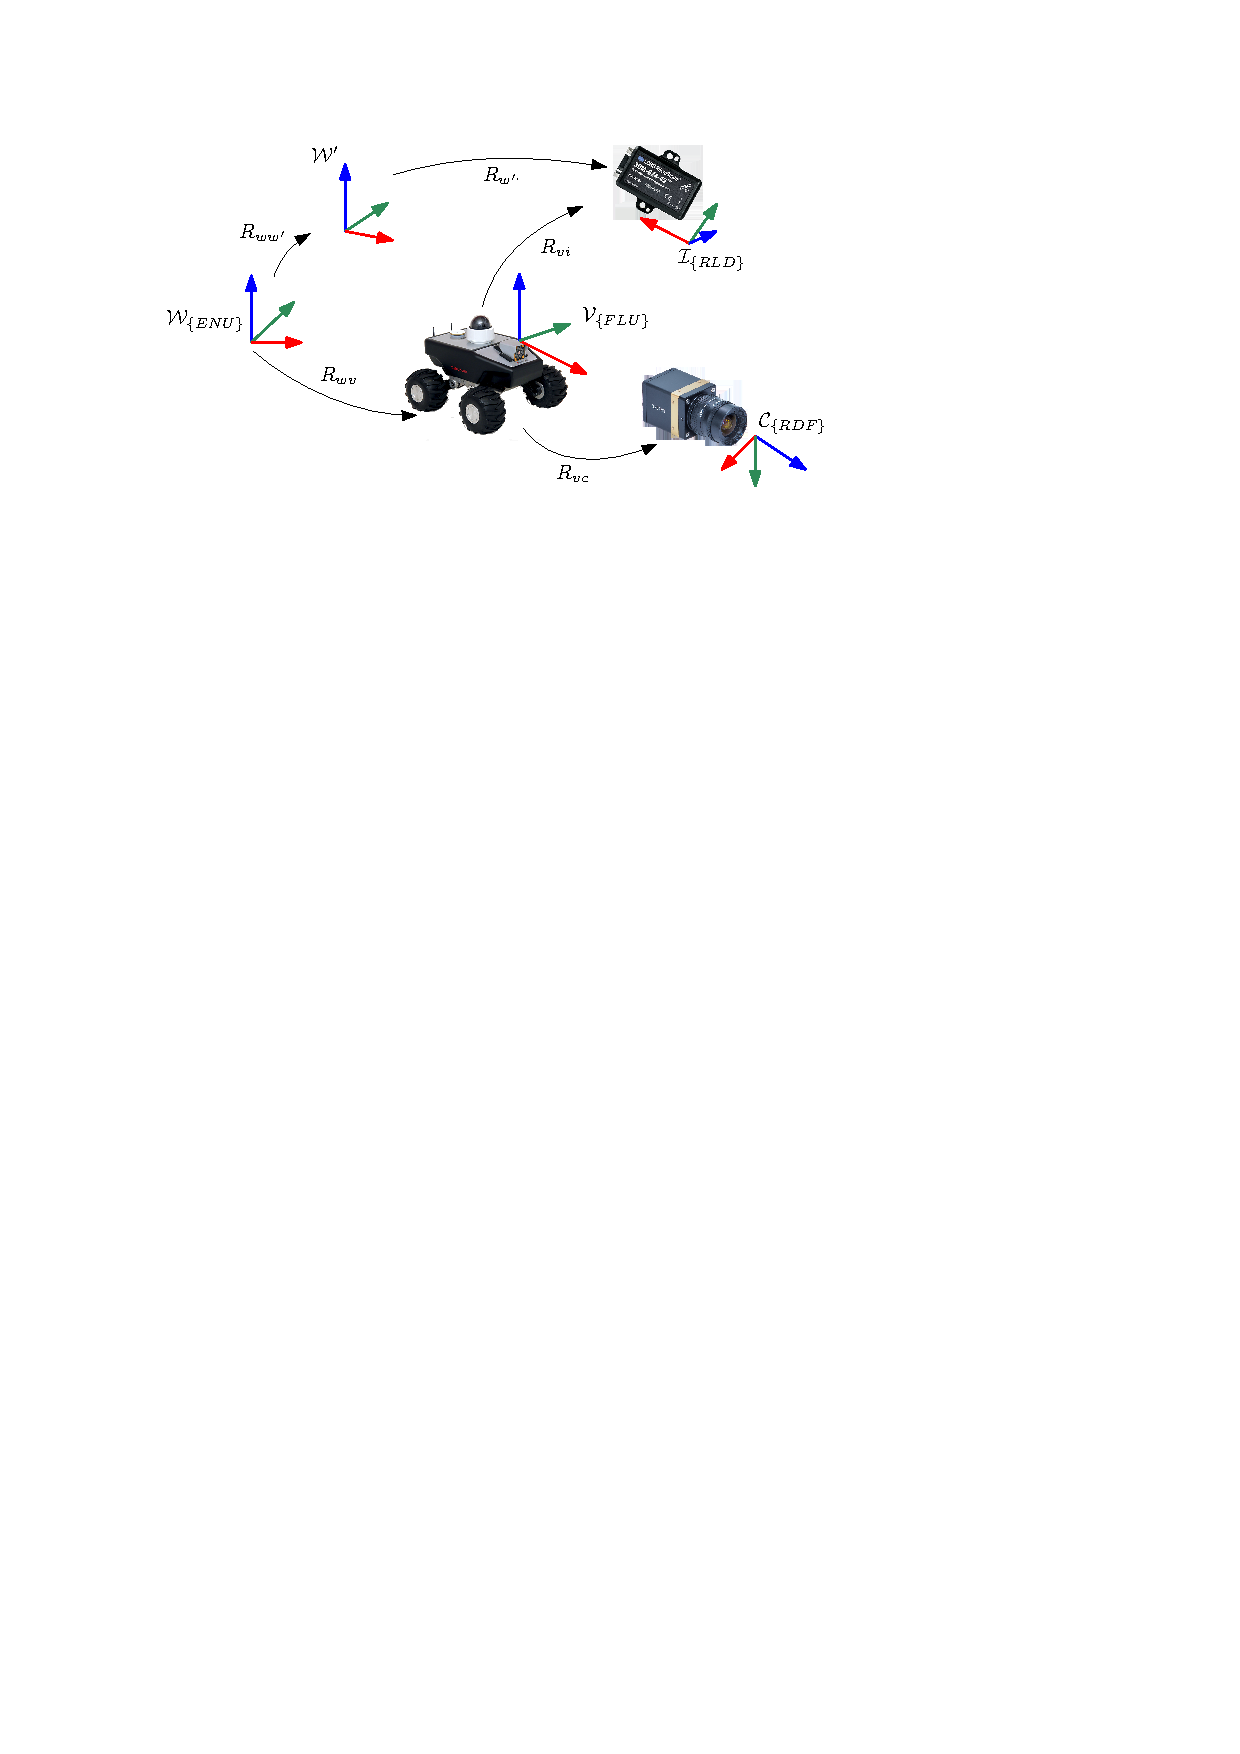
\includegraphics[bb=0bp 0bp 475bp 189bp,width=0.9\paperwidth,draft, type=eps]{../conventions.pdf}
\par\end{centering}
\caption{Frame conventions and notation.}
\end{figure}
\begin{itemize}
\item A vector $y$ expressed in the Pixel Frame $\mathcal{P}$ can be expressed
in the World Frame $\mathcal{W}$ according to:
\begin{align*}
x & =R_{wv}\cdot R_{vc}\cdot R_{cp}\cdot y\\
 & =R\cdot R_{cp}\cdot y
\end{align*}
\item The rotation matrix $R_{cp}$ is defined by:
\[
R_{cp}=\left[\begin{array}{ccc}
\cos\theta_{c}\cos\phi_{c} & -\sin\phi_{c} & \sin\theta_{c}\cos\phi_{c}\\
\cos\theta_{c}\sin\phi_{c} & \cos\phi_{c} & \sin\theta_{c}\sin\phi_{c}\\
-\sin\theta_{c} & 0 & \cos\theta_{c}
\end{array}\right]=R_{z_{c}}(\phi_{c})\cdot R_{y_{c}}(\theta_{c})
\]
\end{itemize}

\subsection*{Relations}

We have:
\begin{equation}
R_{wv}(t)=R_{ww'}\cdot R_{w'i}(t)\cdot R_{vi}^{t}.\label{eq:Rgt_definition}
\end{equation}
Let define the rotation matrix $R$ according to:

\begin{align}
R(t) & =R_{wv}(t)\cdot R_{vc},\label{eq:R_definition}\\
 & =R_{ww'}\cdot R_{w'i}(t)\cdot R_{vi}^{t}\cdot R_{vc}.
\end{align}

\begin{figure}[!h]
\begin{centering}
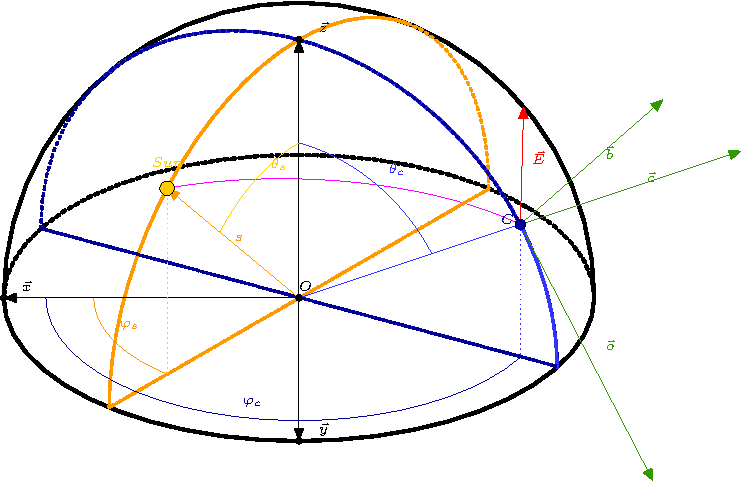
\includegraphics[width=16cm]{polasky4-crop}
\par\end{centering}
\caption{Skylight polarization\label{fig:Skylight-polarization.}.}

\end{figure}

\section{Polarization by scattering}

Using Rayleigh model, the Electric field is orthogonal to the scattering
plane defined by vectors $s$ and $c$. Therefore the normalized Electric
field vector $E$ is given by:
\begin{equation}
E=\frac{s\wedge c}{\left\Vert s\wedge c\right\Vert }\label{eq:E}
\end{equation}
During experiments, the Electric field $E$ vector is measured in
the Pixel frame $\mathcal{P}$:
\begin{equation}
E_{obc}=\left[\begin{array}{l}
E_{o}\\
E_{b}\\
0
\end{array}\right]=\left[\begin{array}{l}
\cos\alpha\\
\sin\alpha\\
0
\end{array}\right]\label{eq:Eproj}
\end{equation}
where $\alpha$ is the measured the angle of polarisation. 

From equation~(\ref{eq:E}) and (\ref{eq:Eproj}) we can write:
\begin{equation}
\begin{cases}
\frac{s\wedge c}{\left\Vert s\wedge c\right\Vert }\cdot o & =E_{o}=\cos\alpha\\
\frac{s\wedge c}{\left\Vert s\wedge c\right\Vert }\cdot b & =E_{b}=\sin\alpha
\end{cases},\label{eq:E0EB vect}
\end{equation}
leading to:

\begin{equation}
\begin{cases}
(s\wedge c)\cdot o & =\left\Vert s\wedge c\right\Vert \cos\alpha\\
(s\wedge c)\cdot b & =\left\Vert s\wedge c\right\Vert \sin\alpha
\end{cases},\label{eq:E0EB vect-1}
\end{equation}
and since$\left\Vert s\wedge c\right\Vert =\left\Vert s\right\Vert *\left\Vert c\right\Vert *\sin\gamma=\sin\gamma$
(with $\gamma$ the angular distance between the observed celestial
point and the sun) we can write:

\begin{equation}
\begin{cases}
(s\wedge c)\cdot o & =\sin\gamma\cos\alpha\\
(s\wedge c)\cdot b & =\sin\gamma\sin\alpha
\end{cases},\label{eq:E0EB vect-1-1}
\end{equation}
The previous system can be rewritten by applying the following rules:

\[
\begin{array}{cl}
\left(s\wedge c\right)\cdot o & =\left(s\wedge\left(o\wedge b\right)\right)\cdot o\\
 & =\left(\left(s\cdot b\right)o-\left(s\cdot o\right)b\right)\cdot o\\
 & =s\cdot b
\end{array},
\]
and

\[
\begin{array}{cl}
\left(s\wedge c\right)\cdot b & =\left(s\wedge\left(o\wedge b\right)\right)\cdot b\\
 & =\left(\left(s\cdot b\right)o-\left(s\cdot o\right)b\right)\cdot b\\
 & =-s\cdot o
\end{array}.
\]
We finally have:
\begin{equation}
\begin{cases}
s\cdot b & =\sin\gamma\cos\alpha\\
s\cdot o & =-\sin\gamma\sin\alpha
\end{cases}\label{eq:scal-b-o}
\end{equation}

The measured degree of polarization is given by {[}pomozi2001{]}:
\begin{equation}
\rho=\rho_{max}*\frac{1-\cos^{2}\gamma}{1+\cos^{2}\gamma}.\label{eq:dop-definition}
\end{equation}
 Consequently, by inverting equation~(\ref{eq:dop-definition}) we
have:
\begin{equation}
\cos\gamma=s\cdot c=\pm\sqrt{\frac{1-\rho'}{1+\rho'}},\label{eq:dop2gamma}
\end{equation}
with $\rho'=\frac{\rho}{\rho_{max}}.$

Expressing the sun vector in the Pixel Frame $\mathcal{P}$ gives
a direct relation between the measured polarization parameters (angle
of polarization $\alpha$ and degree of polarization $\rho$ directly
related to $\gamma$) and the sun position and the celestial point:
\begin{equation}
R^{t}\cdot s=R_{cp}\left[\begin{array}{c}
-\sin\gamma\sin\alpha\\
\sin\gamma\cos\alpha\\
\cos\gamma
\end{array}\right]=v,\label{eq:qtrans}
\end{equation}
where $v$ is a vector obtained from polarization measurements according
to the selected pixel. 

\section{Polarization by reflection with an horizontal surface}

The Electric field is orthogonal to the incidence plane defined by
vectors $c$ and $z=[0,0,1]$. Therefore the normalized Electric field
vector $E$ is given by:
\begin{equation}
E=\frac{z\wedge c}{\left\Vert z\wedge c\right\Vert }\label{eq:E-1}
\end{equation}
Applying the same blabla as in section 1 we obtain:

\begin{equation}
R^{t}\cdot\left[\begin{array}{l}
0\\
0\\
1
\end{array}\right]=R_{cp}\cdot\left[\begin{array}{c}
-\sin\gamma\sin\alpha\\
\sin\gamma\cos\alpha\\
\cos\gamma
\end{array}\right]=w.\label{eq:qtrans-1}
\end{equation}
where $\alpha$ and $\delta$ are respectively the measured angle
of polarization and the angular distance between $c$ and $z$. $\gamma$
is also equal to the angle of incidence (assuming a specular reflection)
and is linked to the measured degree of polarization and the refractive
index of the media using Fresnel properties.

\section{Estimating $\gamma$ }

Assuming that we are only measuring the angle of polarization $\alpha$
in scattering effects, we have to estimate $\gamma$ to get the vector
$v$ defined in eq(\ref{eq:qtrans}). Note that the same method can
be appplied in the case of the reflection to get the vector $w$.

The equation~(\ref{eq:qtrans}) is valid for two different celestial
points $c_{1}$ and $c_{2}$:
\begin{equation}
\begin{cases}
R^{t}\cdot s=R_{cp_{1}}\cdot\left[\begin{array}{c}
-\sin\gamma_{1}\sin\alpha_{1}\\
\sin\gamma_{1}\cos\alpha_{1}\\
\cos\gamma_{1}
\end{array}\right]\\
R^{t}\cdot s=R_{cp_{2}}\cdot\left[\begin{array}{c}
-\sin\gamma_{2}\sin\alpha_{2}\\
\sin\gamma_{2}\cos\alpha_{2}\\
\cos\gamma_{2}
\end{array}\right]
\end{cases}\label{eq:2setseq}
\end{equation}
so we can write:
\begin{equation}
R^{t}\cdot s=R_{cp_{1}}\cdot\left[\begin{array}{c}
-\sin\gamma_{1}\sin\alpha_{1}\\
\sin\gamma_{1}\cos\alpha_{1}\\
\cos\gamma_{1}
\end{array}\right]=R_{cp_{2}}\cdot\left[\begin{array}{c}
-\sin\gamma_{2}\sin\alpha_{2}\\
\sin\gamma_{2}\cos\alpha_{2}\\
\cos\gamma_{2}
\end{array}\right]\label{eq:2points1}
\end{equation}
The equation(\ref{eq:2points1}) can be rewritten according to:

\[
R_{cp_{1}}\cdot\left[\begin{array}{ccc}
\cos\alpha_{1} & -\sin\alpha_{1} & 0\\
\sin\alpha_{1} & \cos\alpha_{1} & 0\\
0 & 0 & 1
\end{array}\right]\left[\begin{array}{c}
0\\
\sin\gamma_{1}\\
\cos\gamma_{1}
\end{array}\right]=R_{cp_{2}}\cdot\left[\begin{array}{ccc}
\cos\alpha_{2} & -\sin\alpha_{2} & 0\\
\sin\alpha_{2} & \cos\alpha_{2} & 0\\
0 & 0 & 1
\end{array}\right]\left[\begin{array}{c}
0\\
\sin\gamma_{2}\\
\cos\gamma_{2}
\end{array}\right]
\]
leading to:
\begin{equation}
M_{1}\cdot\left[\begin{array}{c}
0\\
\sin\gamma_{1}\\
\cos\gamma_{1}
\end{array}\right]=M_{2}\cdot\left[\begin{array}{c}
0\\
\sin\gamma_{2}\\
\cos\gamma_{2}
\end{array}\right]\label{eq:2pts}
\end{equation}
Since the angles of polarization $\alpha_{1},\,\alpha_{2}$ are known
for the 2 points, $M_{1}$ and $M_{2}$ are known and $\gamma_{1},\,\gamma_{2}$
can be found by solving (\ref{eq:2pts}). It can be rewritten according
to:
\[
M_{2}^{t}\cdot M_{1}\left[\begin{array}{c}
0\\
\sin\gamma_{1}\\
\cos\gamma_{1}
\end{array}\right]=\left[\begin{array}{c}
0\\
\sin\gamma_{2}\\
\cos\gamma_{2}
\end{array}\right].
\]
If we denote the matrix $M$ defined such that $M=M_{2}^{t}\cdot M_{1}$,
we have :
\begin{equation}
\begin{cases}
\gamma_{1}=-\arctan\frac{M_{02}}{M_{01}}\\
\gamma_{2}=-\arctan\frac{M_{20}}{M_{10}}
\end{cases}\label{eq:determination-of-gamma}
\end{equation}

The determination of vectors $v$ or $w$ impose to have $\alpha$
and $\gamma$ defined respectively $\pi$ and $2\pi$ modulus or defined
respectively $2\pi$ and $\pi$ modulus. Without loss of generality,
it can be imposed that $\gamma$ (that represents the angle of scattering
or the angle of reflection) is determined in the range $[0,\pi]$
and $\alpha$ is determined in the range $[-\frac{\pi}{2},\frac{3\pi}{2}]$.
Consequently, eq(\ref{eq:2pts}) must be solved considering the four
possible cases :
\[
\left(\alpha_{1},\alpha_{2}\right),\,\left(\alpha_{1},\alpha_{2}+\pi\right),\,\left(\alpha_{1}+\pi,\alpha_{2}\right),\,\left(\alpha_{1}+\pi,\alpha_{2}+\pi\right).
\]
To compute $v$ or $w$, this can be reduced to two solutions:
\begin{equation}
\left(\alpha_{1},\gamma_{1}\right)\,\text{and}\,\left(\alpha_{1}+\pi,-\gamma_{1}\right).\label{eq:candidatesgamma}
\end{equation}
 

\section{Rotation estimation}

\subsection{Absolute rotation}

\subsubsection*{Assumptions}
\begin{itemize}
\item Sun position $s$ is known
\item From 2 measurements of the angle of polarization from the blue sky,
$v$ can be estimated satisfying:
\begin{equation}
s=R(t)\cdot v(t)\label{eq:sun_only}
\end{equation}
 
\item From 2 measurements of the angle of polarization from reflection by
horizontal surface (area of water), $w$ can be estimated satisfying:
\begin{equation}
z=R(t)\cdot w(t)\label{eq:water_only}
\end{equation}
\end{itemize}

\subsubsection*{Derivation}

Using the cross product between (\ref{eq:sun_only}) and (\ref{eq:water_only})
we have the third equation:
\begin{equation}
s\wedge z=R(t)\cdot v(t)\wedge w(t),\label{eq:cross-prod}
\end{equation}
leading to the following system:
\begin{equation}
\begin{cases}
\left[s,z,s\wedge z\right] & =R(t)\cdot\left[v(t),w(t),v(t)\wedge w(t)\right]\\
 & =R_{wv}(t)\cdot R_{vc}\cdot\left[v(t),w(t),v(t)\wedge w(t)\right]
\end{cases}.\label{eq:linear_equation}
\end{equation}
Solving equation (\ref{eq:linear_equation}) enables to get $R_{wv}(t)$
if the sun position $s$ is known.

\subsubsection*{Solving ambiguities}

For each measurment we have in fact two candidates as described in
eq(\ref{eq:candidatesgamma}) providing 2 vectors $v_{1},v_{2}$ and
2 vectors $w_{1},w_{2}$.

Since the angle $\gamma$ in $w_{1}$and $w_{2}$ represents the angle
of reflection must be less than $90{^\circ}$ and it imposes only
one solution regarding $w$.

(NEXT TO BE WRITTEN)

\subsection{Relative rotation}

We can apply formula (\ref{eq:linear_equation}) at 2 different times
$t_{1}$ and $t_{2}$:

\[
\begin{cases}
\left[s,z,s\wedge z\right] & =R_{wv}(t_{1})\cdot R_{vc}\cdot\left[v(t_{1}),w(t_{1}),v(t_{1})\wedge w(t_{1})\right]\\
\left[s,z,s\wedge z\right] & =R_{wv}(t_{2})\cdot R_{vc}\cdot\left[v(t_{2}),w(t_{2}),v(t_{2})\wedge w(t_{2})\right]
\end{cases}.
\]
To simplify the representation let rewrite it according to:
\[
\begin{cases}
\left[s,z,s\wedge z\right] & =R_{wv1}\cdot R_{vc}\cdot\left[v_{1},w_{1},v_{1}\wedge w_{1}\right]\\
\left[s,z,s\wedge z\right] & =R_{wv2}\cdot R_{vc}\cdot\left[v_{2},w_{2},v_{2}\wedge w_{2}\right]
\end{cases}.
\]
So we obtain:
\[
\begin{cases}
\left[s,z,s\wedge z\right] & =R_{wv1}\cdot R_{vc}\cdot\left[v_{1},w_{1},v_{1}\wedge w_{1}\right]\\
R_{wv2} & =\left[s,z,s\wedge z\right]\cdot\left[v_{2},w_{2},v_{2}\wedge w_{2}\right]^{-1}\cdot R_{vc}^{t}\cdot
\end{cases}
\]
And finally:
\begin{equation}
R_{wv2}=R_{wv1}\cdot R_{vc}\cdot\left[v_{1},w_{1},v_{1}\wedge w_{1}\right]\cdot\left[v_{2},w_{2},v_{2}\wedge w_{2}\right]^{-1}\cdot R_{vc}^{t}.\label{eq:relative_equation}
\end{equation}
The relative rotation $R_{v1v2}=R_{wv1}^{T}\cdot R_{wv2}$ is therefore
equal to:

\begin{equation}
R_{v1v2}=R_{vc}\cdot\left[v_{1},w_{1},v_{1}\wedge w_{1}\right]\cdot\left[v_{2},w_{2},v_{2}\wedge w_{2}\right]^{-1}\cdot R_{vc}^{t}\label{eq:final-relative}
\end{equation}

\appendix

\section{ROS coordinate Frame conventions}

Defined in \href{http://www.ros.org/reps/rep-0103.html}{REP 103},
all coordinate frames should follow these conventions.

\subsection*{Chirality}

All systems are right handed. This means they comply with the right
hand rule.

\subsection*{Axis Orientation}

In relation to a body the standard is:
\begin{itemize}
\item x Forward
\item y Left 
\item z Up
\end{itemize}
For short-range Cartesian representations of geographic locations,
use the east north up {[}5{]} (ENU) convention:
\begin{itemize}
\item X East
\item Y North
\item Z Up
\end{itemize}
To avoid precision problems with large float32 values, it is recommended
to choose a nearby origin such as your system's starting position.

\subsection*{Suffix Frames}

In the case of cameras, there is often a second frame defined with
a \char`\"{}\_optical\char`\"{} suffix. This uses a slightly different
convention:
\begin{itemize}
\item x Right 
\item y Down
\item z Forward
\end{itemize}
For outdoor systems where it is desireable to work under the north
east down (NED) convention, define an appropriately transformed secondary
frame with the \char`\"{}\_ned\char`\"{} suffix:
\begin{itemize}
\item X North
\item Y East
\item Z Down
\end{itemize}

\subsection*{Rotation Representation}

There are many ways to represent rotations. The preferred order is
listed below, along with rationale.
\begin{enumerate}
\item quaternion
\begin{itemize}
\item Compact representation
\item No singularities
\end{itemize}
\item rotation matrix 
\begin{itemize}
\item No singularities
\end{itemize}
\item fixed axis roll, pitch, yaw about X, Y, Z axes respectively
\begin{itemize}
\item No ambiguity on order 
\item Used for angular velocities
\end{itemize}
\item euler angles yaw, pitch, and roll about Z, Y, X axes respectively
\begin{itemize}
\item Euler angles are generally discouraged due to having 24 'valid' conventions
with different domains using different conventions by default.
\end{itemize}
\end{enumerate}
By the right hand rule, the yaw component of orientation increases
as the child frame rotates counter-clockwise, and for geographic poses,
yaw is zero when pointing east.

This requires special mention only because it differs from a traditional
compass bearing, which is zero when pointing north and increments
clockwise. Hardware drivers should make the appropriate transformations
before publishing standard ROS messages.

\begin{comment}

\appendix

\section{Appendices}

Let be $K$ the calibration matrix of the camera:

	
\[
K=\left(\begin{array}{ccc}
\alpha_{x} & 0 & u_{0}\\
0 & \alpha_{y} & v_{0}\\
0 & 0 & 1
\end{array}\right)
\]

We have:

\[
\left(\begin{array}{c}
u\\
v\\
w
\end{array}\right)=K\cdot\left(\begin{array}{c}
X\\
Y\\
Z
\end{array}\right)
\]

The pixels coordinate are given by:

\[
\begin{cases}
u & =\alpha_{x}\frac{X}{Z}+u_{0}\\
v & =\alpha_{y}\frac{Y}{Z}+v_{0}
\end{cases}
\]

And therefore:
\[
\begin{cases}
X & =\frac{u-u_{0}}{\alpha_{x}}Z\\
Y & =\frac{v-v_{0}}{\alpha_{y}}Z
\end{cases}
\]

Computation of the 3D ray in the spherical coordinates gives:

\[
\phi=\arctan2\left(\frac{v-v_{0}}{\alpha_{y}},\,\frac{u-u_{0}}{\alpha_{x}}\right)
\]
 and: 

\[
\theta=\arccos\frac{Z}{\sqrt{X^{2}+Y^{2}+Z^{2}}}
\]

\[
\theta=\arccos\frac{1}{\sqrt{\left(\frac{u-u_{0}}{\alpha_{x}}\right)^{2}+\left(\frac{v-v_{0}}{\alpha_{y}}\right)^{2}+1}}
\]
\end{comment}

\end{document}
